\documentclass[11pt,A4]{article}
\usepackage{ctex}
\usepackage{amsmath,mathrsfs,bbding}
\usepackage{siunitx}
\usepackage{diagbox}
\usepackage{amssymb}
\usepackage{amsthm}
\usepackage{indentfirst}
\usepackage[normalem]{ulem} % prevent underlining for biblatex
\usepackage{cases}
\usepackage{lscape}
\usepackage{graphicx}
\usepackage{CJK}
\usepackage{caption}
\usepackage{slashed}
\usepackage{pifont}
\usepackage{float}
\usepackage{booktabs}
\usepackage{makecell}
\usepackage{ulem}
\usepackage{pifont}
\usepackage{enumerate}
\usepackage{ulem}
\usepackage{gensymb}
\usepackage{setspace}
\usepackage{multirow}
\usepackage{subfigure} 
\usepackage{longtable}
\usepackage{cite}
\usepackage[backend=biber]{biblatex}
\addbibresource{sample.bib} %Import the bibliography file
\usepackage{breakcites}
%\setlength{\parindent}{1em}
\usepackage{geometry}
\usepackage{listings} 
\usepackage{xcolor}
\usepackage{color}
\usepackage{xcolor}
\definecolor{dkgreen}{rgb}{0,0.6,0}
\definecolor{gray}{rgb}{0.5,0.5,0.5}
\definecolor{mauve}{rgb}{0.58,0,0.82}

\lstset{frame=tb,
	language=Java, % 使用的语言
	aboveskip=3mm,
	belowskip=3mm,
	showstringspaces=false, % 仅在字符串中允许空格
	backgroundcolor=\color{yellow!10},   % 选择代码背景,必须加上\ usepackage {color}或\ usepackage {xcolor}
	columns=flexible,
	basicstyle = \ttfamily\small,
	frame = shadowbox,  
	numbers=left, % 给代码添加行号,可取值none, left, right.
	numberstyle=\small \color{gray},  % 行号的字号和颜色
	keywordstyle=\color{blue},
	commentstyle=\color{dkgreen}, % 设置注释格式
	stringstyle=\color{mauve},
	breaklines=true,   % 设置自动断行.
	breakatwhitespace=true, % 设置是否当且仅当在空白处自动中断.
	escapeinside=``, %逃逸字符(1左面的键),用于显示中文
	frame=shadowbox, %设置边框格式
	extendedchars=false, %解决代码跨页时,章节标题,页眉等汉字不显示的问题
	xleftmargin=2em,xrightmargin=2em, aboveskip=1em, %设置边距
	tabsize=4 % 将默认tab设置为4个空格
}

\geometry{top=2.54cm,bottom=2.54cm,left=3cm,right=3cm}

%\usepackage{array}
%\usepackage{booktabs}
\renewcommand{\baselinestretch}{1.5}
%\usepackage{subeqnarray}

%\usepackage[ruled]{algorithm2e}
\usepackage{algorithmicx,algorithm}
\usepackage{algpseudocode}
%\usepackage{amssymb}
\renewcommand{\algorithmicrequire}{\textbf{Input:}} 
\renewcommand{\algorithmicensure}{\textbf{Output:}}
\newcommand{\xizhi}[1]{{\color{red} xizhi: #1}}
\begin{document}

\title{{\bigskip\bigskip\bigskip\bigskip\bigskip\bigskip\bigskip\bigskip\bigskip\bigskip\bigskip\Huge The title}\bigskip\bigskip}

\author{
 Teng Jiang \\ UNI: tj2488
}

\bigskip

\maketitle
\newpage
\tableofcontents
\newpage

\section{TODO}

Strongly typed: 
能不能override:能!Variable overriding

constructor (non-primitive type definition的问题)

Func和Struct有syntactic sugar,不使用function了
\begin{lstlisting}
// Func
最后一个是return type,前面是input type, semantics时候检查对应不对应
Func<input1 type, input 2 type,..., return type> s = new Func (int x)->int {...} 
Func s = func (int x)->int {...}
Func s = (int x)->int {...}
func s (int x)->int {...} // syntactic sugar
? Func s (int x)->int {...} // syntactic sugar
BUT NOT
Func s;
s (int x)->int {...} // no good
Func f = (int) -> int;

// String
String s = new String "abc";
String s = string "abc";
String s = "abc";
string s "abc"; // syntactic sugar

// Struct
Struct s = new Struct {int a; Func<int,int> f;};
Struct s = struct {int a; Func<int,int> f;};
Struct s = {int a; Func<int,int> f;};
struct s {int a; Func<int,int> f;}; // syntactic sugar

// Array
Array<int> a = new Array<int> [1,2,3];
Array<int> a = array [1,2,3];
Array<int> a = [1,2,3];
array<int> a [1,2,3];

\end{lstlisting}


TLDR: Teng 3.15的update
1. 关于new和delete,以及元素在heap上->Java风格
2. 关于func和function
3. 关于type的大小写(primitive vs non primitive)
4. Good way to present code: https://dev.to/niharrs/6-awesome-ways-to-present-your-code-3jj2
5. 如果什么都不return,return Null?

Irene 3.17 Updates
1. 不忍心改这个,建了一个新的file,见左边sdraft.tex
2. 在做statements
3. working...struggling...working...

\begin{lstlisting}
/* bubbleSort.csm */

struct MyObject {
    int index;
    String text;
}

function compareMyObject(MyObject a, MyObject b)->bool {
    return a.index < b.index;
}

function bubbleSort(Array<MyObject> arr, int n,
    func compare(MyObject, MyObject)->bool)->Array<MyObject>
{
    for (int i = 0; i < n - 1; i++) {
        for (int j = 0; j < n - i - 1; j++) {
            if (compare(arr[j], arr[j + 1])) {
                MyObject temp = arr[j];
                arr[j] = arr[j + 1];
                arr[j + 1] = temp;
            }
        }
    }
    return arr;
}

/* Declaration and definition of myArray and n omitted */

bubbleSort(myArray, n, compareMyObject);

/* Also we need to free all elements, so we should have a function that does all clean up*/
\end{lstlisting}

Clean up example: https://www.cs.columbia.edu/~sedwards/classes/2021/4115-spring/reports/C-net.pdf
Example Code 2: client-server.cnet (cnet)
\begin{lstlisting}
struct conn{
string serv_addr;
int port;
string req_fname;
file f;
socket sock;
};
void cleanup(struct conn client_conn)
{
delete client_conn.sock;
delete client_conn.f;
delete client_conn;
return;
}
\end{lstlisting}

要不要function overwriting
Typing system? 要不要parametric typing?
Scope... (回看第一版proposal的要求)
https://github.com/AjayMT/silk

https://verigu.github.io/4115Spring2024/assignments/lrm.html
https://www.cs.columbia.edu/~sedwards/classes/2018/4115-fall/lrms/Shoo.pdf
https://go.dev/ref/spec
https://www.cs.columbia.edu/~sedwards/classes/2018/4115-fall/lrms/Coral.pdf
https://www.cs.columbia.edu/~sedwards/classes/2017/4115-spring/lrms/Pipeline.pdf
https://www.cs.columbia.edu/~sedwards/classes/2015/4115-fall/lrms/Dice.pdf
https://www.cs.columbia.edu/~sedwards/classes/2014/w4115-fall/lrms/FRY.pdf
https://www.cs.columbia.edu/~sedwards/classes/2017/4115-fall/reports/WebLang.pdf
https://www.cs.columbia.edu/~sedwards/classes/2021/4115-spring/reports/C-net.pdf
https://www.cs.columbia.edu/~sedwards/classes/2021/4115-spring/reports/Go--.pdf

Cnet里面说:我觉得我们不要做garbage collection,就用free就好了
https://www.cs.columbia.edu/~sedwards/classes/2021/4115-spring/reports/C-net.pdf
Furthermore, C-net discards the complex semantics of dynamic
memory allocation in C by abstracting pointers for the user. As a result, most data on C-net is
stored on the heap, except for primitives and the references to the objects, similar to the Java
programming language. In addition, C-net provides a highly intuitive and convenient interface to
strings that is used for all I/O operations and automatically allocated/freed without explicit
invocations from the programmer. For non-primitive objects except strings, however, C-net does
not have automatic garbage collection and therefore the user is required to free all allocated
objects, although the semantics for allocating and freeing objects is quite straightforward

我觉得这个make sense

In Java, arrays are objects, and like all objects in Java, they reside on the heap. When you create an array in Java using the new keyword, memory is allocated from the heap to store the elements of the array. The reference to the array itself can be stored either on the stack (if it's a local variable) or on the heap (if it's an instance variable or a static variable). However, the actual array data is always stored on the heap.

Boolean operators in this language are: == (checks for equality) , != (checks for inequality), <,
>, >=, <=. The last four operate on int and float types only. and != also work for strings,
arrays and structs. For strings, these two operators work on string equality, that is, are the two
strings the same length and comprised of the same characters in the same order. For structs
and arrays however, the two operators check the equality of the memory reference, that is, do
the arrays or structs refer to the same underlying array or struct?


要不要支持Socket/File/Struct
要不要支持overloading
https://levelup.gitconnected.com/first-class-functions-in-golang-ef2a5001bb4f

% \begin{lstlisting}
% struct MyObject {
%     int index;
%     int data;
% }

% function compareData(MyObject a, MyObject b)->bool {
%     return a.data < b.data;
% }

% function bubbleSort(Array<MyObject> arr, int n, func compare(MyObject, MyObject)->bool)->Array<MyObject> {
%     for (int i = 0; i < n - 1; i++) {
%         for (int j = 0; j < n - i - 1; j++) {
%             if (compare(arr[j], arr[j + 1])) {
%                 MyObject temp = arr[j];
%                 arr[j] = arr[j + 1];
%                 arr[j + 1] = temp;
%             }
%         }
%     }
%     return arr;
% }
% \end{lstlisting}
1231231231312321313123312321312131232131231233213123123212312321323123213312332
A segment of an example Cesame program:
\begin{lstlisting}[caption={bubbleSort.csm}, captionpos=b]
function bubbleSort(Array<MyObject> arr, int n, func compare(MyObject, MyObject)->bool)->Array<MyObject> {
    for (int i = 0; i < n - 1; i++) {
        for (int j = 0; j < n - i - 1; j++) {
            if (compare(arr[j], arr[j + 1])) {
                MyObject temp = arr[j];
                arr[j] = arr[j + 1];
                arr[j + 1] = temp;
            }
        }
    }
    return arr;
}
\end{lstlisting}


Arrays are implemented by mallocing the memory needed for the array and then returning
the pointer to the malloc’d array.
If the array contains composite types, the elements need to be initialized independently. Arrays
initialized using new will not have any initialization performed on the elements. If the array is
defined with literals, the items will already be initialized. For primitive types, the actual values
will be stored, for composite types like structs, other arrays, strings, or functions, a reference
to the element is stored instead of the value itself.

Pass by value and pass by reference
https://stackoverflow.com/questions/40480/is-java-pass-by-reference-or-pass-by-value

Typing:
We should have primitive types and non-primitive types.

Primitive types are not capitalized: int, float, func, string...

Non-primitive types are capitalized: String, Array

参考Javascript/Typescript的typing

https://developer.mozilla.org/en-US/docs/Web/JavaScript/Reference/Global_Objects/String#string_primitives_and_string_objects

function 是function definition
func是function declaration
    
Func as a type

Irene: 
- Statements
- operator and Arithmetic
- control flow

Teng:
- Function
- printf

Qian:
Array
Struct

\section{Overview}

Something.

\section{Introduction}

Something.


\section{Problem Formulation}

Something.



\subsection{Problem Definition}

Some example:

\begin{itemize}
    \item \textbf{Aggregate Column}, also called aggregated column. It refers to the only column to which we apply our aggregation functions (SUM, AVG, MAX, MIN, ...).
    \item \textbf{Grouping Columns}, also called group-by columns. They are the columns that can be put in the GROUP BY clause. These columns are used to categorize and organize the data into groups based on their unique values.
    \item \textbf{Number of Columns, denoted with $N$}: The total number of the column(s) we can perform GROUP BY on. 
    \item \textbf{Dimension, denoted with $D$}: The actual number of the column(s) we will GROUP BY on. 
    \item \textbf{Cardinality, denoted with $K$}: We assume that all GROUP BY columns have the same cardinality. Cardinality means the number of unique values of a column.
\end{itemize}

In this report, we focus on blah. A code block


\lstset{language=SQL}
\lstset{breaklines=true}
\begin{lstlisting}
SELECT SUM(AggregateColumn)
FROM TABLE
GROUP BY GroupingColumn_n_1, GroupingColumn_n_2, ..., GroupingColumn_n_D
\end{lstlisting}

\subsection{UPMEM Introduction}

A figure:

\begin{figure}[H]
\centering
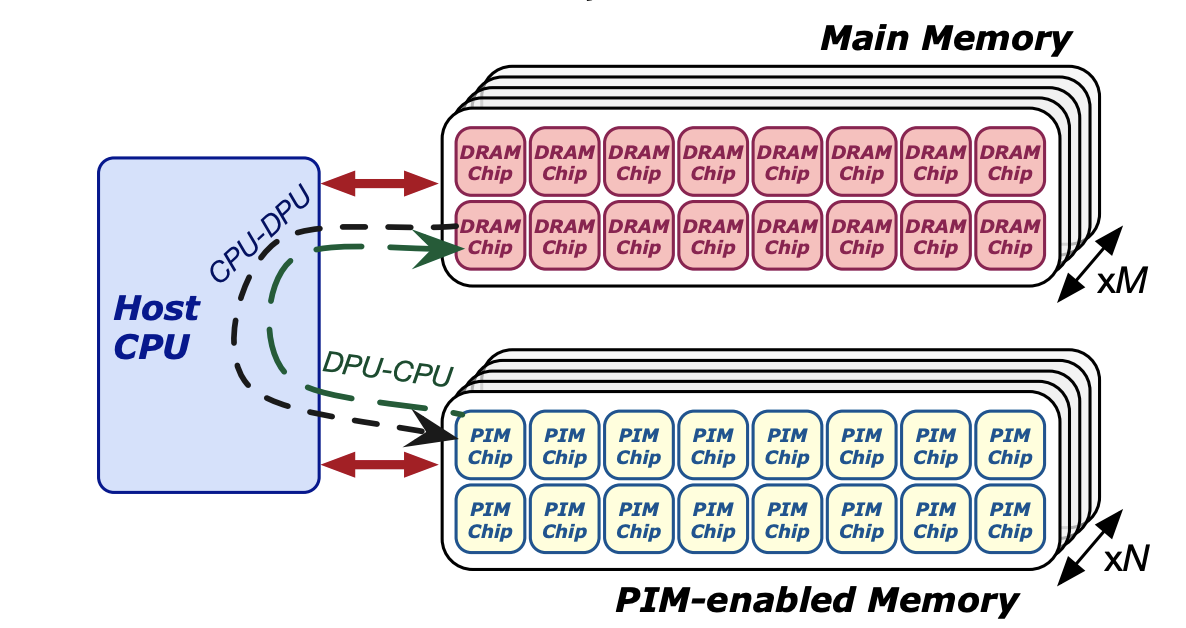
\includegraphics[scale=0.60]{UPMEM.png}
\caption{Illustration of CPU-DPU Data Transfer in UPMEM Cloud.}
\end{figure}


\subsection{Strategy}





\section{Code Breakdown}
code

\lstset{language=C}
\lstset{breaklines=true}
\begin{lstlisting}
// Initialize semaphores to 1, meaning they are free to grab
sem_init(&sem[0], 0, 1);
sem_init(&sem[1], 0, 1);

// Create threads
pthread_create(&tid_writer, NULL, send_tuples, &send_args);
pthread_create(&tid_reader, NULL, fill_tuples, &fill_args);

// Join threads
pthread_join(tid_writer, NULL);
pthread_join(tid_reader, NULL);

// Destroy semaphores
sem_destroy(&sem[0]);
sem_destroy(&sem[1]);
\end{lstlisting}


\subsection{More code}



\lstset{language=C}
\lstset{breaklines=true}
\begin{lstlisting}
void* send_something(void* send_args) { // launch
    
    pthread_exit(NULL);
}
\end{lstlisting}




\section{Function}
One of the most important features

We are using xxx



\subsection{Comparison: Different Data Distributions}

$$
\begin{aligned}
&\textbf{Table 2: Execution Time of Different Data Distributions (sec)}\\
&\begin{tabular}{lrrr}
\hline & \multicolumn{3}{c}{Data Distribution} \\
\cline { 2 - 4 } Variable & Even & Uneven (70\%) & More Uneven (90\%) \\
\hline With xxx & 0.113004 & 0.324721 & 0.428407 \\
Without xxx & 0.115473 & 0.338165 & 0.435363\\
\hline
\end{tabular}
\end{aligned}
$$


\section{Acknowledgment}

I want to acknowledge xxx



% $$
\printbibliography[
heading=bibintoc,
] %Prints the entire bibliography with the title "Whole bibliography"
\end{document}


\lstlistoflistings
